\newpage
\section{SIMULADORES} \label{simuladores}

\subsection{La Central Nuclear José Cabrera y el SGIZ}

Tal y como se ha comentado en la introducción del proyecto, se pretende profundizar en el conocimiento de los \emph{\acrlongpl{smr}} mediante la simulación de la operación de una central nuclear con un comportamiento muy similar al de un \acrshort{smr}: la Central Nuclear de José Cabrera, también conocida como Central Nuclear de Zorita.

\subsubsection{La Central Nuclear de Zorita}

La Central Nuclear José Cabrera está situada en Almonacid de Zorita (Guadalajara) y fue la primera central nuclear española en operación.

Se trata de un \textbf{reactor de agua a presión (\acrshort{pwr})} diseñado por Westinghouse. Este tipo de reactores emplea agua ligera como refrigerante y moderador, trabajando con neutrones en el rango térmico para maximizar la tasa de fisión del $U^{235}$, presente en un 3,3\% ---en el caso de la central nuclear de Zorita--- del Uranio Enriquecido (UE) empleado como combustible.

La central comenzó a construirise en julio de 1965. Tras 36 meses de construcción, el 31 de marzo de 1968 se realizó la prueba funcional en caliente y en junio de ese mismo año se hizo la carga del núcleo, alcanzando su primera criticidad. La red eléctrica española comenzó a recibir los primeros kilovatios-hora de origen nuclear el 14 de julio de 1968 y, desde entonces, se inició un aumento gradual de potencia que llevó a la explotación comercial de la central, con una \textbf{potencia eléctrica instalada de 150 MWe} y una \textbf{potencia térmica de 510 MWt}. El titular de su explotación fue Unión Fenosa Generación (actualmente Naturgy). Durante 39 años de operación comercial produjo 36.515 millones de kWh, empleando a 300 trabajadores de forma directa y a unos 6.000 de forma indirecta.

\begin{figure}[h]
    \centering
    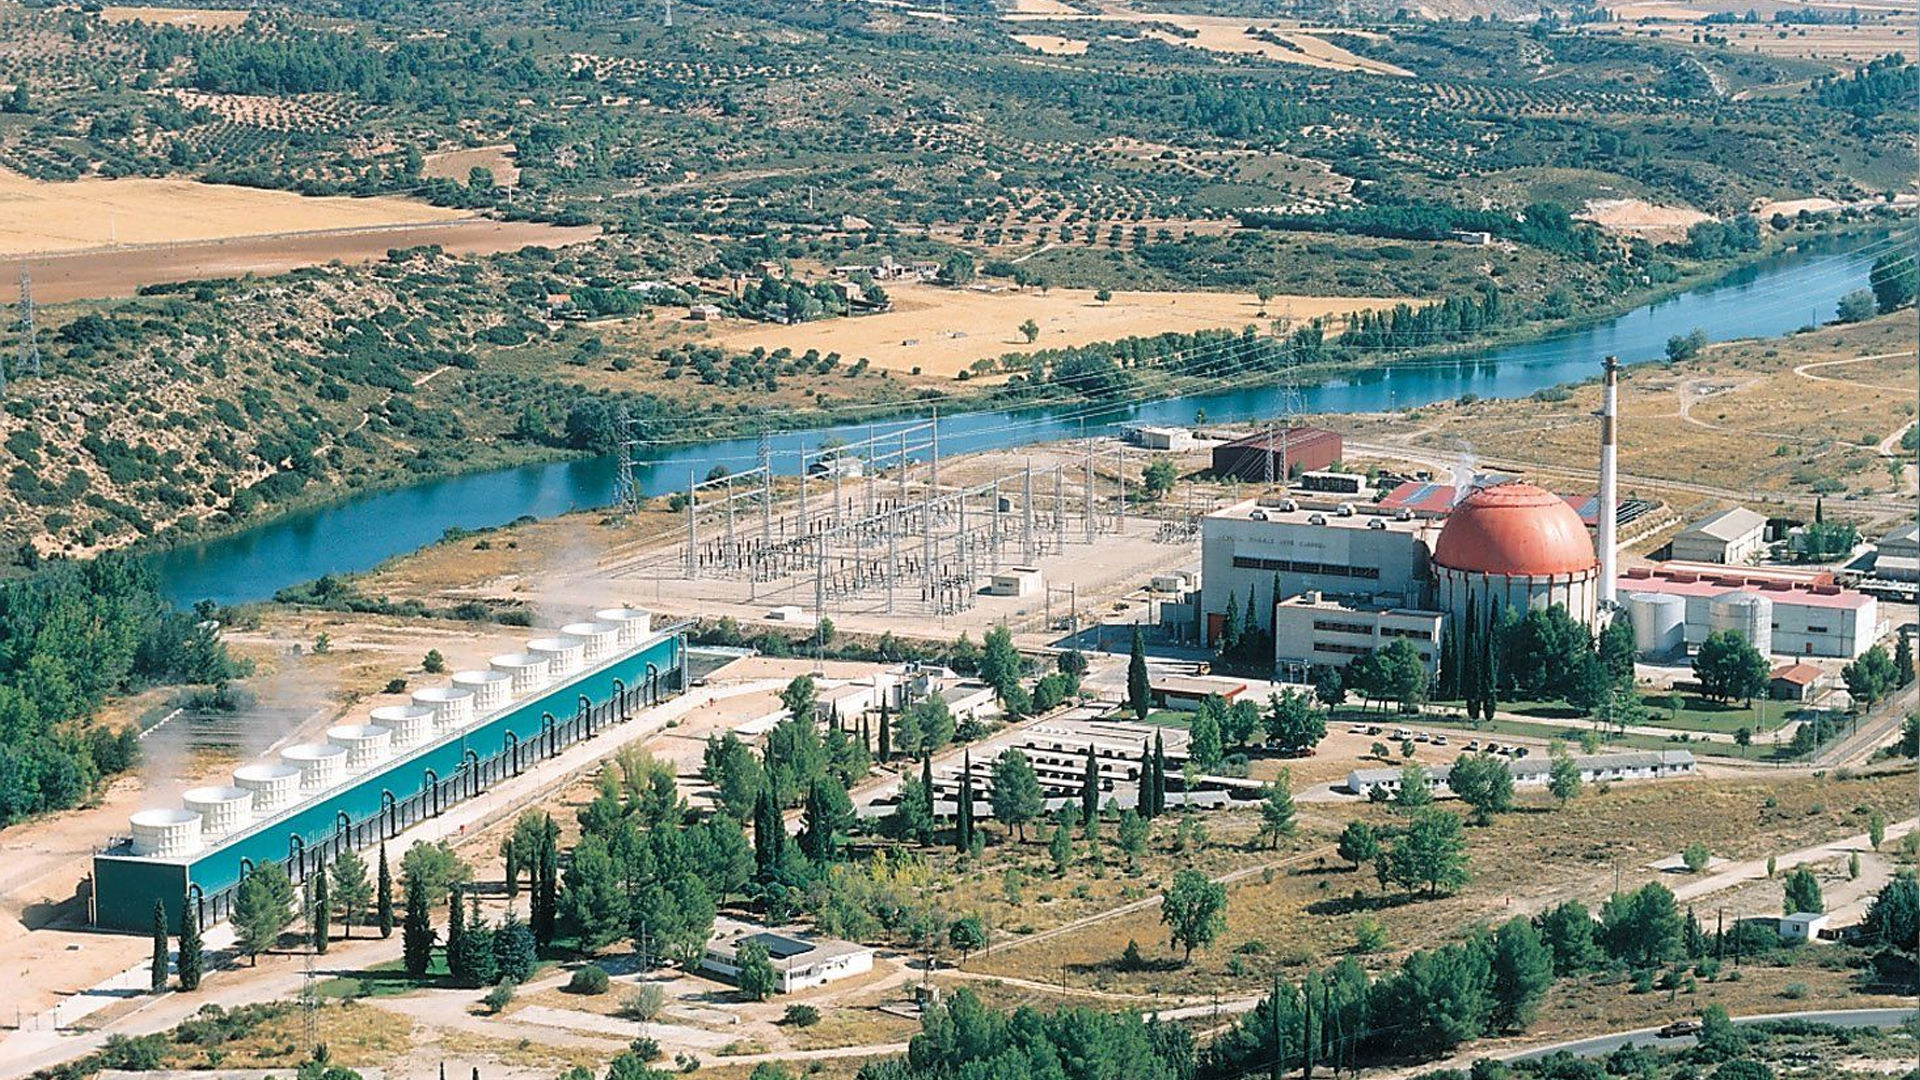
\includegraphics[width=\textwidth]{content/figures/zorita.jpg}
    \caption{Central Nuclear José Cabrera (\cite{sne_recursos_prensa}).}
    \label{fig:zorita}
\end{figure}

El cese definitivo de explotación de la central fue declarado por el Ministerio de Industria, Turismo y Comercio mediante la Orden Ministerial del 20 de abril de 2006. El titular de las actividades de desmantelamiento de la central es \acrshort{enresa}, por lo que se tubo que cambiar la titularidad de la instalación de Gas Natural Fenosa a \acrshort{enresa}. El 11 de febrero de 2010, \acrshort{enresa} inició el desmantelamiento de la instalación.

La alternativa escogida fue un desmantelamiento total e inmediato en un horizonte temporal de unos ocho años. Las actividades de desmantelamiento comprenden también la segmentación mediante técnicas de corte especiales de grandes sistemas y componentes radiológicamente significativos, como el generador de vapor y la vasija del reactor, así como la descontaminación y demolición de edificios y la restauración final del emplazamiento. 

Actualmente, la instalación se encuentra en la fase de restauración, en la cual se pretende devolver al emplazamiento a sus condiciones previas a la construcción de la central, saneando todo el terreno en cuestión. Los elementos de combustible irradiado de la central se están almacenando temporalmente en el \acrfull{ati} de la instalación, en el que también se han depositado algunos residuos generados durante el desmantelamiento (\cite{enresa_desmantelamiento_zorita}).

En la siguiente tabla se resume lo más importante de lo expuesto anteriormente sobre la central nuclear de Zorita:

\begin{table}[h]
    \resizebox{\textwidth}{!}{%
    \begin{tabular}{|cc|cl|cc|}
    \hline
    \rowcolor[HTML]{ECF4FF} 
    \multicolumn{2}{|c|}{\cellcolor[HTML]{ECF4FF}\textbf{Localización}} &
      \multicolumn{2}{c|}{\cellcolor[HTML]{ECF4FF}\textbf{Propiedad}} &
      \multicolumn{1}{c|}{\cellcolor[HTML]{ECF4FF}\textbf{Titular}} &
      \textbf{Tipo} \\ \hline
    \multicolumn{2}{|c|}{Almonacid de Zorita (Guadalajara)} & \multicolumn{2}{c|}{Unión Fenosa (Naturgy)} & \multicolumn{1}{c|}{Enresa}      & PWR    \\ \hline
    \rowcolor[HTML]{ECF4FF} 
    \multicolumn{1}{|c|}{\cellcolor[HTML]{ECF4FF}\textbf{Potencia térmica}} &
      \textbf{Potencia eléctrica} &
      \multicolumn{2}{c|}{\cellcolor[HTML]{ECF4FF}\textbf{Refrigeración}} &
      \multicolumn{2}{c|}{\cellcolor[HTML]{ECF4FF}\textbf{Autorización construcción}} \\ \hline
    \multicolumn{1}{|c|}{510 MWt}         & 160 MWe         & \multicolumn{2}{c|}{Abierta - Río Tajo}                & \multicolumn{2}{c|}{24 de junio de 1964}  \\ \hline
    \rowcolor[HTML]{ECF4FF} 
    \multicolumn{2}{|c|}{\cellcolor[HTML]{ECF4FF}\textbf{Autorización de puesta en marcha}} &
      \multicolumn{2}{c|}{\cellcolor[HTML]{ECF4FF}\textbf{Cese de explotación}} &
      \multicolumn{2}{c|}{\cellcolor[HTML]{ECF4FF}\textbf{Autorización desmantelamiento}} \\ \hline
    \multicolumn{2}{|c|}{11 de octubre de 1968}             & \multicolumn{2}{c|}{30 de abril de 2006}               & \multicolumn{2}{c|}{1 de febrero de 2010} \\ \hline
    \end{tabular}%
    }
    \caption{Características y fechas clave de la Central Nuclear José Cabrera (\cite{csn_info_zorita}).}
    \label{tabla:resumen_zorita}
    \end{table}

\subsubsection{Comparación de la Central Nuclear de Zorita con un SMR}

Pendiente...

\subsubsection{El Simulador Gráfico Interactivo de Zorita (SGIZ)}

El \acrshort{sgiz} es un simulador gráfico interactivo de alcance total de la Central Nuclear de Zorita. Durante los años de operación de la central, se empleó para el entrenamiento de los operadores de la sala de control, para comprender y analizar la dinámica de la planta y para desarrollar y validar sus procedimientos operativos de emergencia.

En abril de 2008 se firmó el convenio de colaboración entre Unión Fenosa y la UPM para la creación del Aula "José Cabrera", donde se instaló el \acrshort{sgiz}. Este aula se ubica en el Departamento de Ingeniería Nuclear de la ETSII-UPM y está dedicada a la enseñanza de la Tecnología de la Operación de las Centrales Nucleares.

El simulador proporciona las respuestas de la planta durante la operación normal, transitorios y condiciones de accidente, basadas en el código TRAC y un conjunto de pantallas ilustrativas en tiempo real, así como un conjunto de alarmas en un panel similar al de la sala de control real de la central nuclear, permitiendo la operación automática y manual en tiempo real de los componentes del sistema completo tanto en condiciones normales como de emergencia.